\documentclass[6pt]{../../shared/AiTex}
\usepackage{csvsimple}

\title{Memoria entrega 1}
\author{A.L.K.}
\date{Febrero 2024}

\begin{document}
%\datos{facultad}{universidad}{grado}{asignatura}{subtitulo}{autor}{curso}
\datos{Informática}{Universidad Complutense de Madrid}{Ingeniería informática}{Aprendizaje Automatico y Big Data}{Entrega 1: regresión lineal de una variable}{Alejandro Barrachina Argudo}{2023-2024}
% \portadaApuntes
% \pagestyle{empty}
% \tableofcontents
% \pagestyle{empty}
\justify

\begin{center}

    {\huge \textbf{\underline{\subtitulo}}} \\
    { \lesson - \autor}

\end{center}


\section*{Introducción}

En este documento se explicará el código del entregable 1 y el proceso de la regresión lineal

Para esta práctica se usarán los siguientes \textit{imports} vistos en la figura \ref{fig:imports}.
\begin{figure}[H]
    \centering
    \lstinputlisting[firstline=1,lastline=6, style=custompython]{../linear_reg.py}
    \caption{Código de las bibliotecas usadas}
    \label{fig:imports}
\end{figure}

\section{Regresión lineal}

Para esta regresión definimos la función de pendiente como en la figura \ref{fig:fun} como métrica, también se usan las funciones de coste \ref{fig:compute_cost} y de gradiente \ref{fig:compute_gradient} según descritas en los apuntes.

Para hacer el gradiente descendente usamos \ref{fig:gradient_descent} con 1500 iteraciones, 0.01 en $\alpha$ y 0 para iniciar w y b.

\begin{figure}[H]
    \centering
    \lstinputlisting[firstline=15,lastline=26, style=custompython]{../linear_reg.py}
    \caption{Código de la función `fun'}
    \label{fig:fun}
\end{figure}

\begin{figure}[H]
    \centering
    \lstinputlisting[firstline=29,lastline=47, style=custompython]{../linear_reg.py}
    \caption{Código de la función `compute\_cost'}
    \label{fig:compute_cost}
\end{figure}

\begin{figure}[H]
    \centering
    \lstinputlisting[firstline=53,lastline=70, style=custompython]{../linear_reg.py}
    \caption{Código de la función `compute\_gradient'}
    \label{fig:compute_gradient}
\end{figure}

\begin{figure}[H]
    \centering
    \lstinputlisting[firstline=76,lastline=110, style=custompython]{../linear_reg.py}
    \caption{Código de la función `gradient\_descent'}
    \label{fig:gradient_descent}
\end{figure}

\section{Gráficas}

Para hacer los gráficos primero tendremos que hacer un \textit{grid} con la función `make\_grid' (figura \ref{fig:make_grid}). Tras esto podemos hacer el contorno (\ref{fig:show_contour}) visto en la figura \ref{fig:contour} y el valle en 3D con `show\_mesh' (figure \ref{fig:show_mesh}) visto en la figura \ref{fig:mesh}.

Para ver la evolución de J(w,b) tenemos el gráfico \ref{fig:history_linear}, pero como en los últimos pasos evoluciona lentamente podemos ver la figura \ref{fig:history_log} con otra escala, hechos con la función `show\_J\_history' \ref{fig:show_J_history}.

\begin{figure}[H]
    \centering
    \lstinputlisting[firstline=113,lastline=134, style=custompython]{../linear_reg.py}
    \caption{Código de la función `make\_grid'}
    \label{fig:make_grid}
\end{figure}

\begin{figure}[H]
    \centering
    \lstinputlisting[firstline=137,lastline=155, style=custompython]{../linear_reg.py}
    \caption{Código de la función `show\_contour'}
    \label{fig:show_contour}
\end{figure}

\begin{figure}[H]
    \centering
    \lstinputlisting[firstline=137,lastline=155, style=custompython]{../linear_reg.py}
    \caption{Código de la función `show\_mesh'}
    \label{fig:show_mesh}
\end{figure}

\begin{figure}[H]
    \centering
    \lstinputlisting[firstline=226,lastline=242, style=custompython]{../linear_reg.py}
    \caption{Código de la función `show\_J\_history'}
    \label{fig:show_J_history}
\end{figure}

\begin{figure}[H]
    \centering
    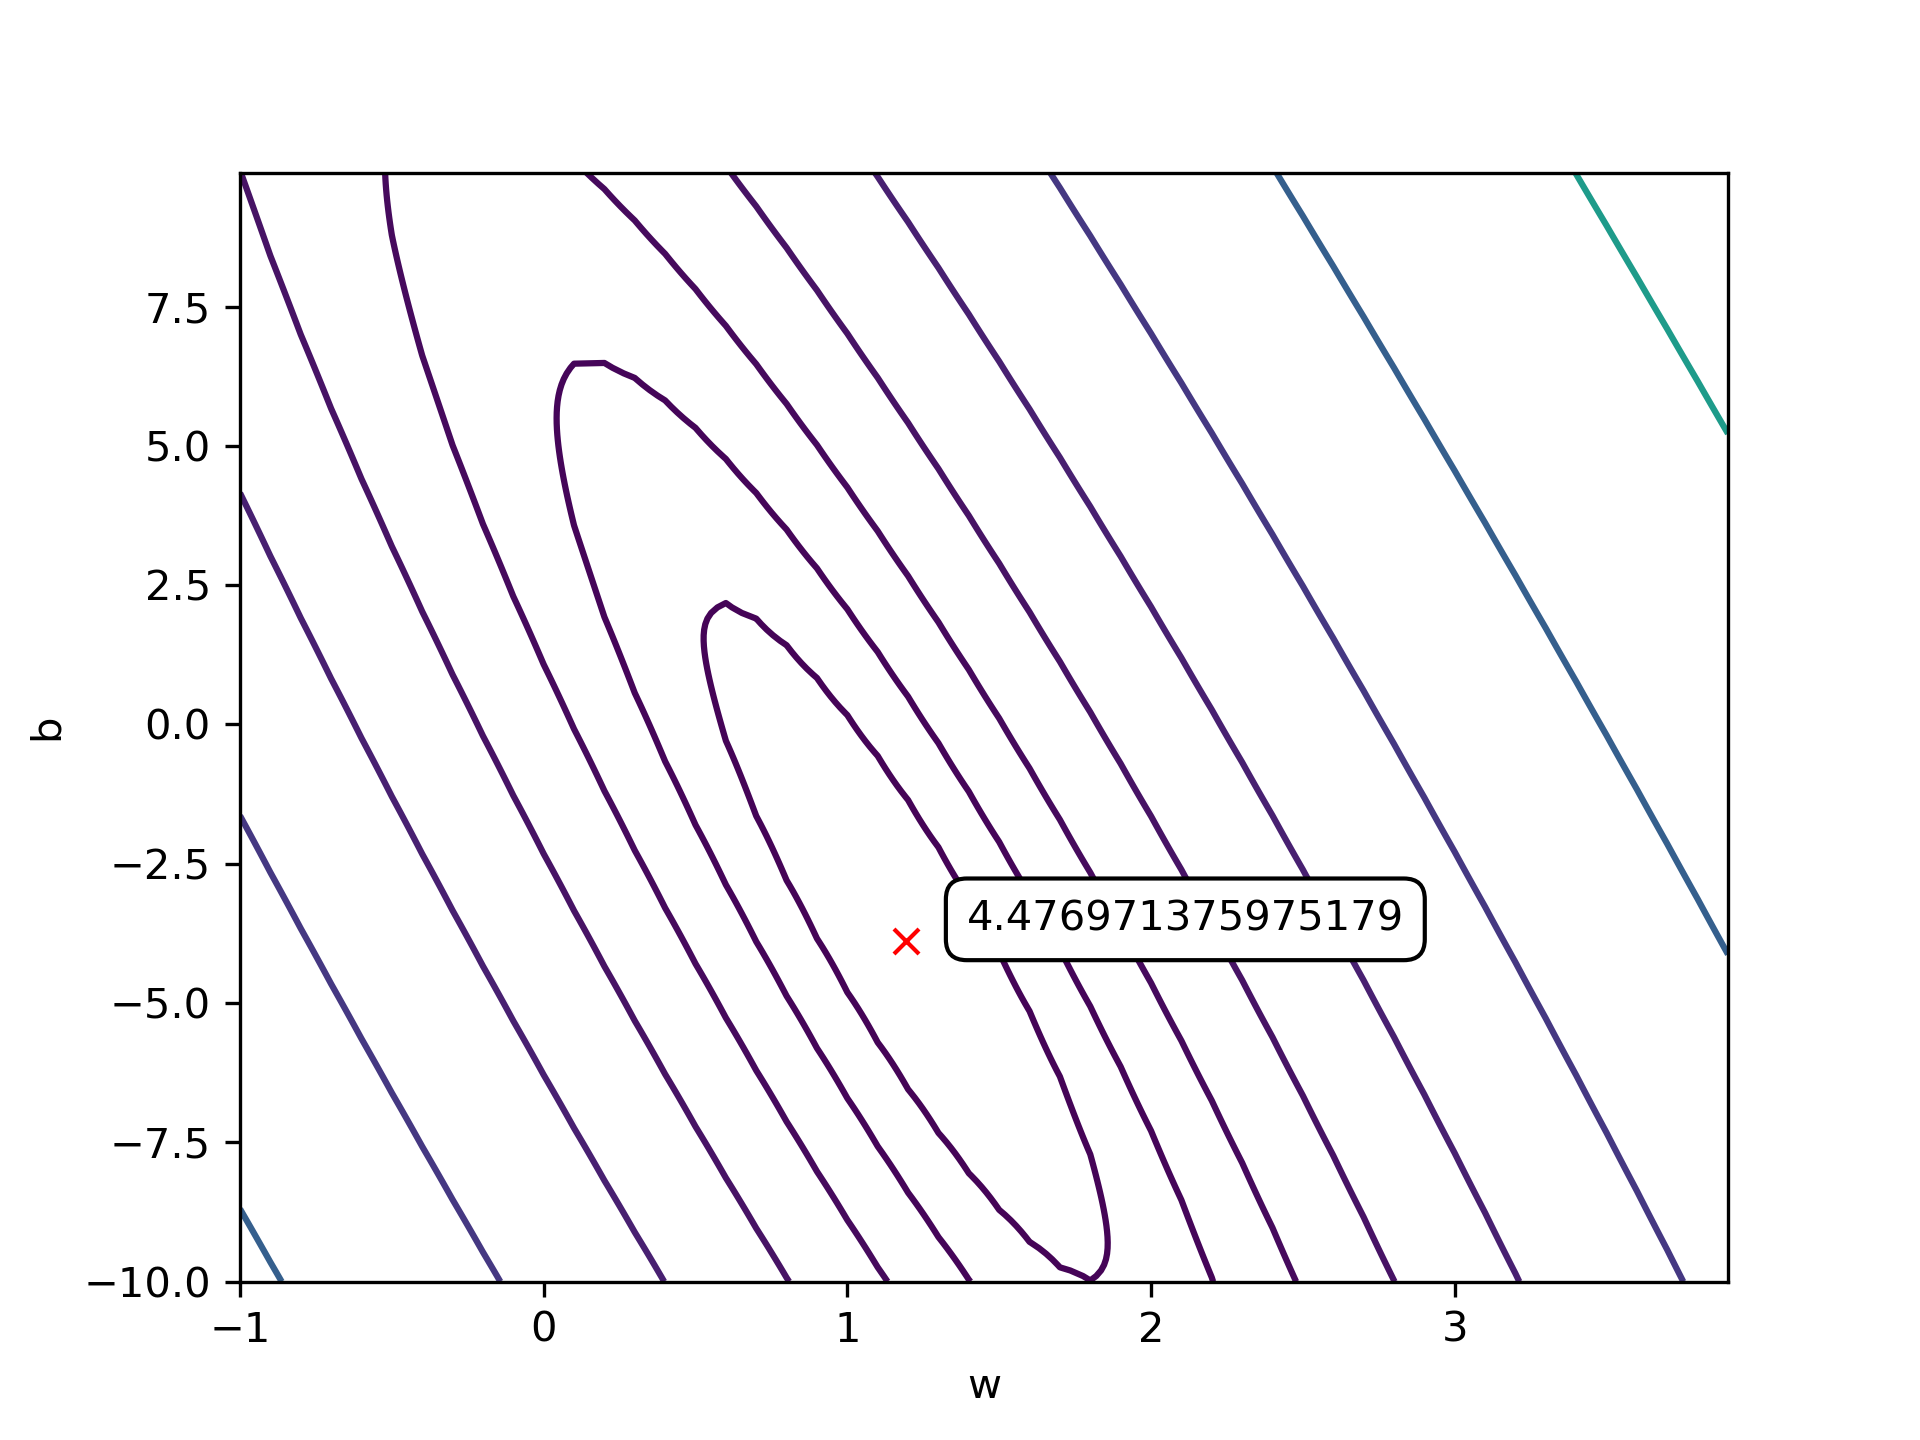
\includegraphics[width=0.6\textwidth]{imagenes/contour_plot.png}
    \caption{Gráfico de contorno}
    \label{fig:contour}
\end{figure}

\begin{figure}[H]
    \centering
    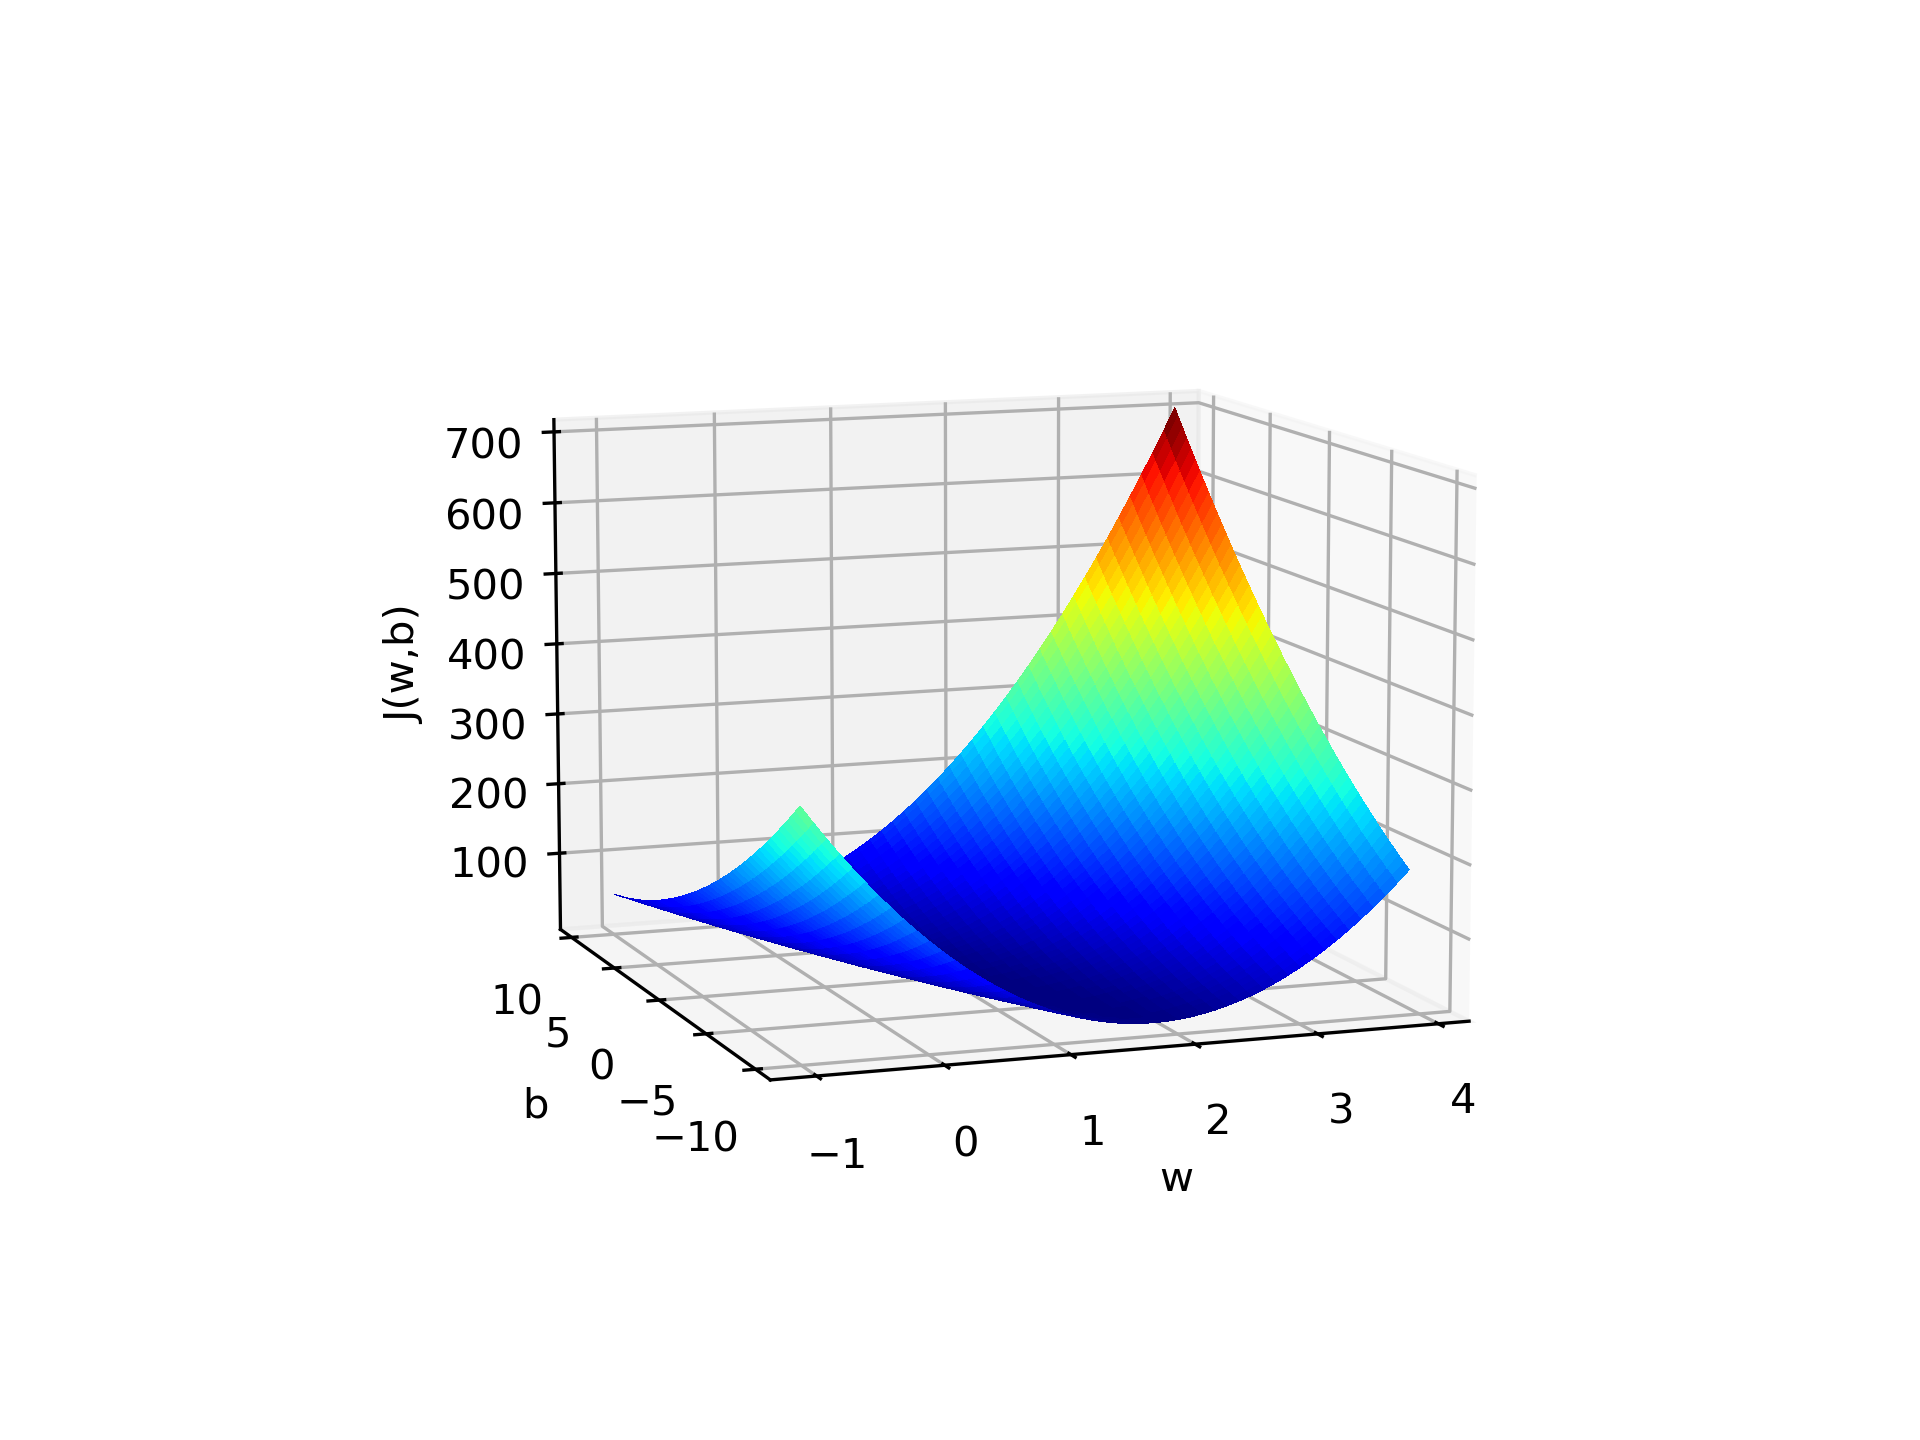
\includegraphics[width=0.6\textwidth]{imagenes/mesh.png}
    \caption{Gráfico de Valle}
    \label{fig:mesh}
\end{figure}

\begin{figure}[H]
    \centering
    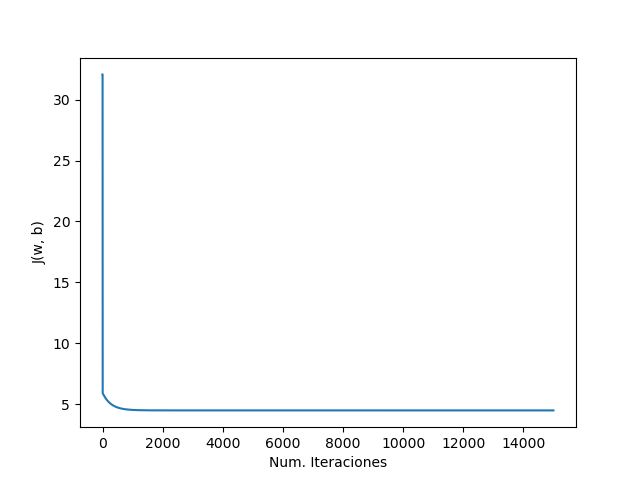
\includegraphics[width=0.6\textwidth]{imagenes/J_history_linear.png}
    \caption{Gráfico de J\_history linear}
    \label{fig:history_linear}
\end{figure}

\begin{figure}[H]
    \centering
    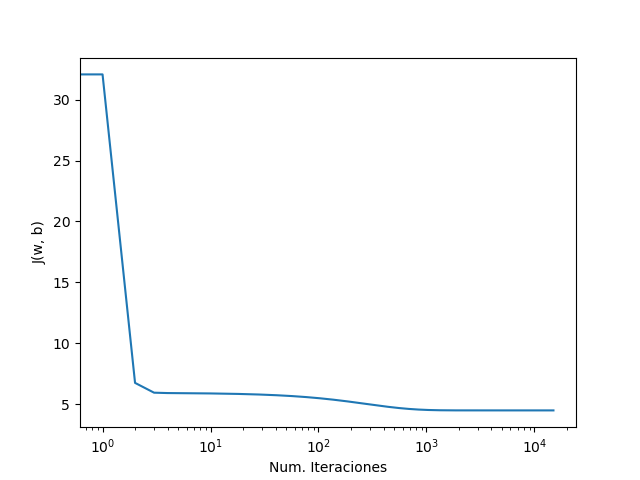
\includegraphics[width=0.6\textwidth]{imagenes/J_history_log.png}
    \caption{Gráfico de J\_history log}
    \label{fig:history_log}
\end{figure}

\section{conclusiones}

Tras todas las iteraciones de `gradient\_descent', nos quedamos con el gráfico \ref{fig:scatter} producido por la función \ref{fig:show_scatter_line}. Podemos ver la línea azul representando la predicción de precios y los puntos rojos representando los datos dados.

Para visualizar los datos de manera numérica usamos la función \ref{fig:write_results}, la cual nos produce un historial simplificado de J(w,b) (tabla \ref{table:j_history}) y las predicciones para 35K personas y 70K personas (tabla \ref{table:predicciones}).

\begin{table}[H]
    \centering
    \csvreader[tabular=|c|r|,
        table head=\hline \textbf{Tam Población} & \textbf{Prediccion} \\ \hline,
        late after line=\\ \hline]
    {./recursos/predicciones.csv}{1=\casos,2=\iterativo}
    {\casos & \iterativo}
    \caption{Predicciones para 35K personas y 70K personas}
    \label{table:predicciones}
\end{table}

\begin{table}[H]
    \centering
    \csvreader[tabular=|c|r|,
        table head=\hline \textbf{Iteraciones} & \textbf{J(w,b)} \\ \hline,
        late after line=\\ \hline]
    {./recursos/j_history_simplificado.csv}{1=\casos,2=\iterativo}
    {\casos & \iterativo}
    \caption{Evolución de J(w,b)}
    \label{table:j_history}
\end{table}

\begin{figure}[H]
    \centering
    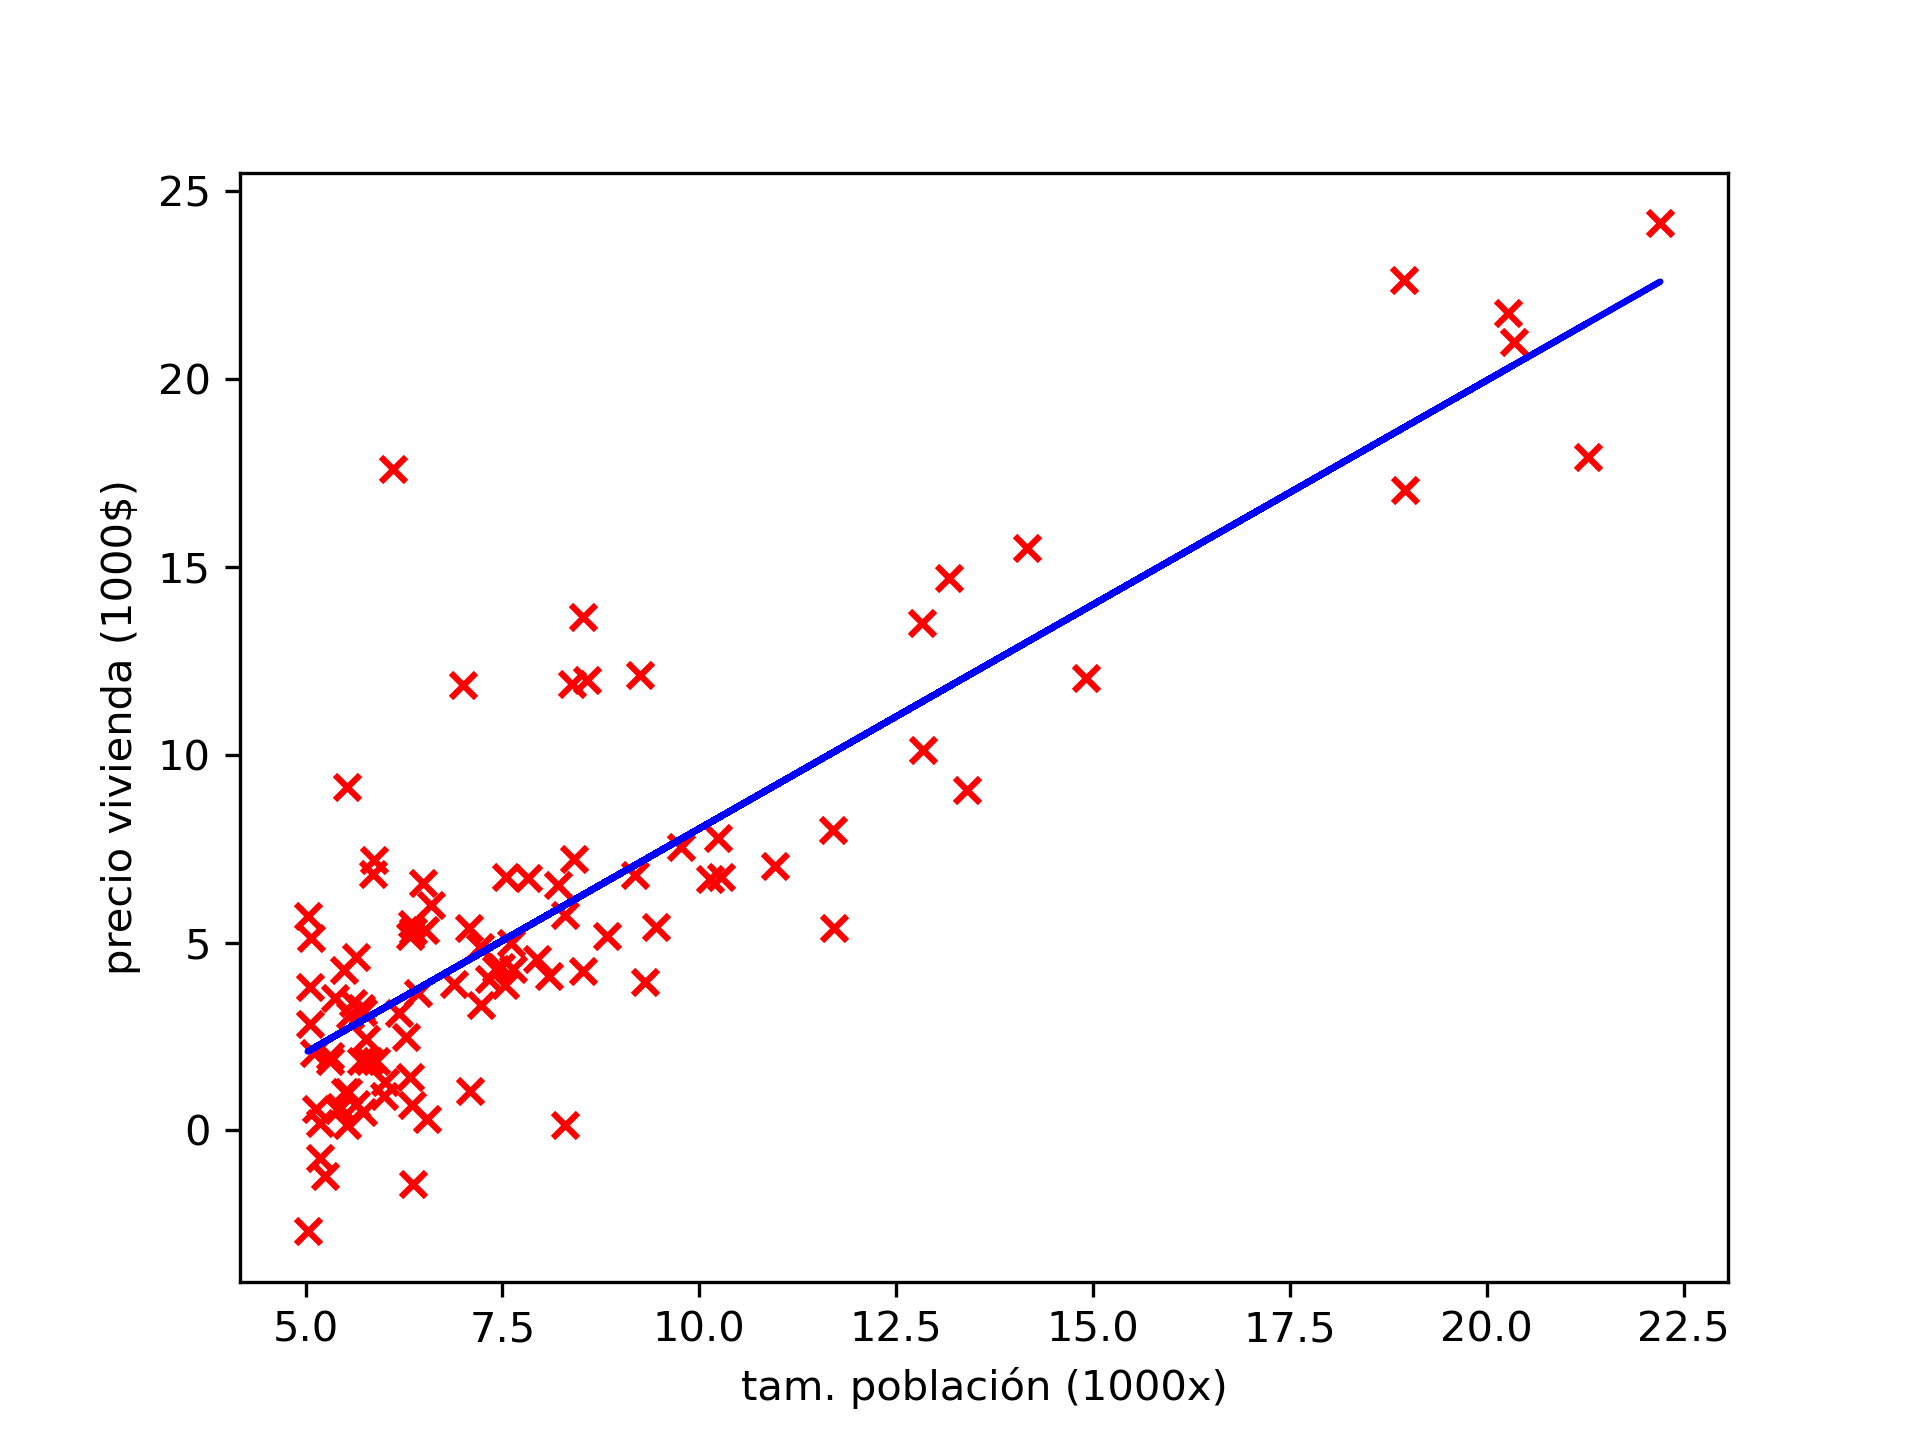
\includegraphics[width=0.6\textwidth]{imagenes/scatter.png}
    \caption{Gráfico de la predicción (azul) y los datos dados (rojo)}
    \label{fig:scatter}
\end{figure}

\begin{figure}[H]
    \centering
    \lstinputlisting[firstline=179,lastline=201, style=custompython]{../linear_reg.py}
    \caption{Código de la función `show\_scatter\_line'}
    \label{fig:show_scatter_line}
\end{figure}

\begin{figure}[H]
    \centering
    \lstinputlisting[firstline=204,lastline=223, style=custompython]{../linear_reg.py}
    \caption{Código de la función `write\_results'}
    \label{fig:write_results}
\end{figure}



\end{document}
